\documentclass{article}
\usepackage{pgfplots}
\usepackage[utf8]{inputenc}

\pagestyle{empty}
%\pgfplotsset{compat=1.17}

\begin{document}

\begin{figure}
    \centering
    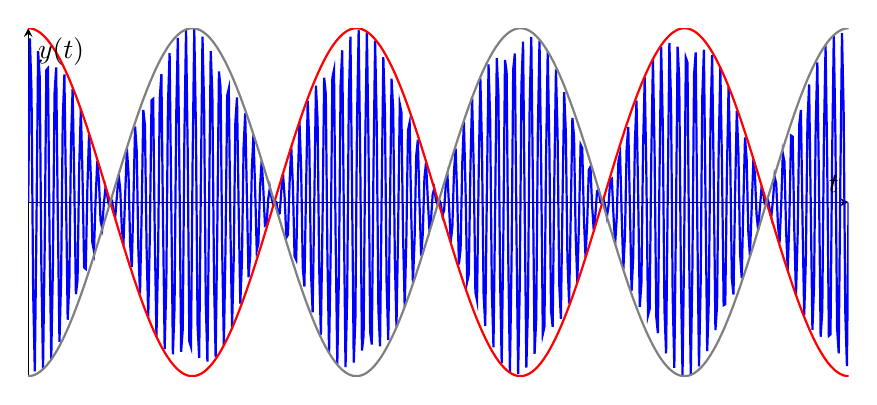
\begin{tikzpicture}
        \begin{axis}[
            xlabel=$t$, ylabel={$y(t)$},
            axis lines=middle,
            grid=none,
            width=12cm, height=6cm,
            xmin=0, xmax=10,
            ymin=-2, ymax=2,
            samples=500,
            domain=0:10,
            xtick=\empty, % Removes x-axis numbers
            ytick=\empty, % Removes y-axis numbers
            ]
            
            % Hochfrequente Schwingung (blau)
            \addplot[blue, thick] {sin(deg(2*pi*10*x)) + sin(deg(2*pi*9.5*x))};
            
            % Obere Hüllkurve (rot)
            \addplot[red, thick, no marks, domain=0:10] {2*cos(deg(0.5*pi*1*x))};
            
            % Untere Hüllkurve (grau)
            \addplot[gray, thick, no marks, domain=0:10] {-2*cos(deg(0.5*pi*1*x))};

        \end{axis}
    \end{tikzpicture}
    Schwebung: Die blaue Kurve ist die hochfrequente Schwingung (Ton), und die roten und grauen Kurven repräsentieren die Hüllkurven der Schwebung (Lautstärke).
\end{figure}

\end{document}
